\documentclass{article}

\usepackage{graphicx}
\usepackage{minted}

\usepackage[dutch]{babel}

\title{ 
\includegraphics[scale=1]{gorilla.png} \\ Code Gorilla \\ Klassendiagrammen}
\author{Dagmar Hofman}
\date{}

\begin{document}
	\maketitle
	\newpage
	\tableofcontents
	\newpage
	\section{Inleiding}
	
	Dit document gaat over klassendiagrammen. \\
	Een klassendiagram toont klasen en hun samenhang. Klassendiagrammen kunnen tijdens analyse, ontwerp en implementatie gebruikt worden. In elke fase wordt alleen datgene in het klassendiagram opgenomen, wat in die fase belangrijk is. Het is dus belangrijk om te weten waarvoor een klassendiagram op een bepaald moment gebruikt wordt. \\
	Tijdens de analyse wordt het domeinmodel opgesteld, waarin de belangrijkste concepten voor het systeem met hun onderlinge relaties worden vastgelegd.
	Bij domeinmodellering bevat het klassendiagram klassen met attributen maar nog zonder methoden. Ook zullen de attributen nog niet voorzien worden van typen (dat is een latere ontwerp- of impementatiekeuze), en hebben de relaties tussen de klassen nog geen richting. \\
	
	\section{De notatie van een klasse}
	
	\bigskip
	
	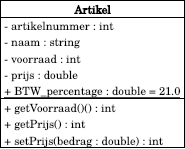
\includegraphics[scale=1.8]{diagram1.png} \\
	Figuur 1. Voorbeeld van een klassediagram.
	
	\newpage
	
	\noindent We bekijken eerst de notatie voor een klasse. In figuur 1 zien we dat het klassendiagram bestaat uit drie delen: \\
	\begin{enumerate}
		\item De naam van de klasse
		\item De attributen van de klasse
		\item De methoden van de klasse
	\end{enumerate}

	Op ontwerpniveau wordt soms geen java-typen (zoals int, string etc.) gebruikt om de typen weer te geven. Men kan ook duidingen zoals 'Geheel getal' of 'Bedrag' en dergelijke gebruiken. \\
	
	Voor attributen hanteerd UML de volgende syntax: \\
	
	\texttt{
	[toegang] naam[: type] [= waarde]
	} \\

\smallskip
	
	\noindent \textit{Toegang} geeft aan of het attribuut behoort tot: \\
	\begin{itemize}
		\item Public	(+)
		\item Private	($-$)
		\item Package	($\sim$)
		\item Protected (\#)
	\end{itemize}
	
	\noindent \textit{Naam} en \textit{Type} geven de naam en het type van het attribuut weer.
	
	\noindent De volledige syntaxis voor methodeduidingen is: \\
	
	\texttt{
	[toegang] naam([parameterlijst]) [: resultaattype]
	} \\

	\smallskip
	

	Voorbeeld: \\
	
	\smallskip
	
	\noindent Een methode voor de klasse order die gebruikt kan worden om de BTW uit te rekenen is dan als volgt: \\

	\begin{minted}{Java}
	+berekenBTW(bedrag: Double): Double
	\end{minted}
	
	Attributen en/of methoden kunnen worden weggelaten uit het diagram. \\
	\newpage
	
	\section{Associaties}
	
	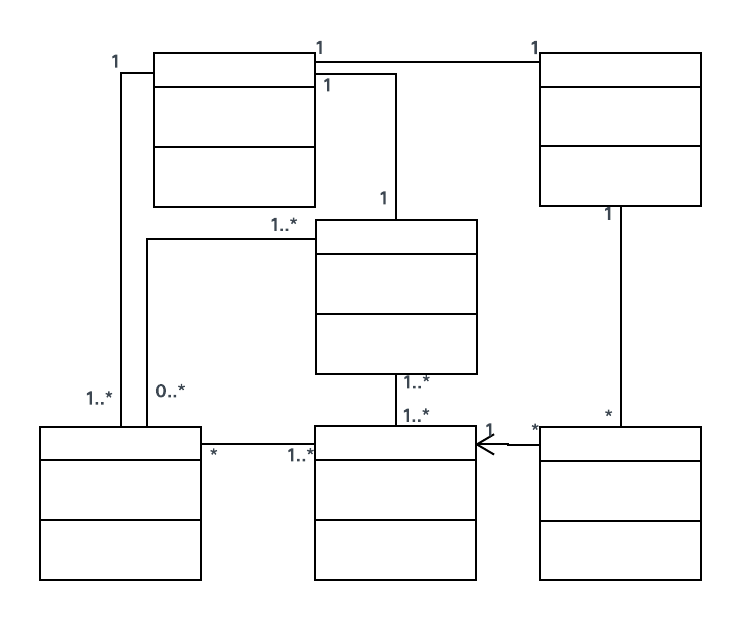
\includegraphics[scale=1]{assoc.png} \\
	Figuur 2. Voorbeeld van associaties bij het klassendiagram.
	
	Bij een \textit{associatie} wordt een klasse als attribuut opgenomen in een andere klasse. \\
	
	Deze kunnen zijn: \\
	
	\begin{enumerate}
		\item \'{E}\'{e}n op \textbf{n} relaties.
		\item \'{E}\'{e}n op meer relaties.
		\item \'{E}\'{e}n op \textbf{n}..\textbf{m} relaties.
		\item \'{E}\'{e}n op \textbf{n} of meer relaties.
		\item Meer op meer relaties.
		\item Meer op \textbf{n}..\textbf{m} relaties.
		\item Meer op \textbf{n} of meer relaties.
		\item Meer op 1 of meer relaties.
	\end{enumerate}
	
	\section{Conclusie}
	
	In dit document wordt weergegeven hoe klassendiagrammen te schrijven.
	
\end{document}          
